\documentclass[sigconf,nonacm]{acmart}
\settopmatter{printacmref=false}
\renewcommand\footnotetextcopyrightpermission[1]{}
\usepackage{booktabs,multirow,array,graphicx}
\usepackage{enumitem}
\usepackage{pdfpages}
\setlist[itemize]{nosep,leftmargin=*}
\setlist[enumerate]{nosep,leftmargin=*}

\title{Evaluating Targeted Data Augmentation for Robust Retail Product Classification Under Image Degradation}
\subtitle{CSE791 Research Methodology and Seminar --- Group 09 (Computer Vision)}
\author{Abdur Rahman Ohi}
\affiliation{\institution{BRAC University}\department{Department of Computer Science and Engineering; Student ID: 22301280}\city{Dhaka}\country{Bangladesh}}
\author{Rafi Ehtesham Mozumder}
\affiliation{\institution{BRAC University}\department{Department of Computer Science and Engineering; Student ID: 22301489}\city{Dhaka}\country{Bangladesh}}
\renewcommand{\shortauthors}{Ohi and Mozumder}
\begin{document}

\begin{abstract}
Fine-grained retail product classification can be unreliable when product images are blurred, darkened, or partly occluded. Although data augmentation is established, its relative benefits depend on the corruption and application. This ongoing comparative study evaluates whether degradation-targeted augmentation offers greater robustness than conventional augmentation without a meaningful reduction in clean-image accuracy. We fine-tuned the same ImageNet-pretrained EfficientNet-B0 with minimal (Basic), RandAugment (Generic), or blur/low-light/occlusion-specific (Targeted) training on a cleaned nine-class subset of the Nyris-hosted Products-10K collection. The pilot contains 427 training, 105 validation, and 54 untouched official test images. Across three training seeds, Targeted achieved 83.81\% mean severe-blur validation accuracy versus 71.75\% for Generic, a 12.06-percentage-point improvement; corresponding clean accuracies were 95.87\% and 96.83\%. The Targeted advantage was smaller for severe low light (+2.54 points) and absent for severe occlusion ($-0.32$ points). These exploratory findings indicate a degradation-dependent trade-off rather than uniform superiority. Exact duplicates were removed, but the limited, mixed-category SKU sample, potential near duplicates, synthetic corruptions, and validation-based checkpoint selection constrain inference. The official test set remains sealed. The contribution is an auditable, severity-aware retail classification comparison rather than a new augmentation algorithm.
\end{abstract}
\keywords{retail SKU classification, EfficientNet-B0, data augmentation, corruption robustness, Products-10K, repeated-seed validation}
\ccsdesc[500]{Computing methodologies~Image representations}
\ccsdesc[300]{Computing methodologies~Computer vision}
\maketitle

\section{Introduction}
\subsection{Motivation and problem statement}
Visual recognition of retail stock-keeping units (SKUs) supports electronic cataloging, assisted checkout and inventory systems. Unlike coarse category recognition, SKU classification can depend on small labels, packaging details and minor design differences. The Products-10K dataset was introduced to study such fine-grained identification across commercial items \cite{bai2020products}. Retail systems now also include retrieval-based few-shot approaches, hierarchical recognition and real-store detection pipelines \cite{lamm2025rag,hori2026hierarchical,sah2026grocer}. Their deployment setting may be affected by motion blur, inadequate illumination, variable viewpoints and partial visibility. In this paper we isolate three such distortions and ask how robust a fixed classifier remains as image quality decreases.

The \emph{problem} is that high classification accuracy on clean e-commerce photographs does not demonstrate dependable recognition under degraded mobile-camera-like inputs. The \emph{research need} is to quantify whether simply matching augmentation to foreseeable corruptions provides a repeatable advantage over standard augmentation for retail SKU recognition, and whether it compromises clean-image accuracy. A model that succeeds only for its training corruption types might fail on other distortions. Similarly, a few-point clean accuracy loss can matter even if selected robustness measures increase.

\subsection{Research questions and hypotheses}
\textbf{RQ1.} How do blur, low illumination and partial occlusion at increasing severity levels affect retail SKU classification accuracy and macro-F1?\\
\textbf{RQ2.} Does targeted degradation-specific augmentation improve corrupted-image accuracy relative to Basic and Generic augmentation with architecture and training budget held fixed?\\
\textbf{RQ3.} Is any robustness advantage accompanied by reduced clean-image accuracy?

The directional working hypotheses are that classification accuracy decreases as degradation strengthens (H1), that the Targeted-versus-Generic difference depends on corruption type (H2), and that their clean-image accuracies need not be equal (H3). These are empirical questions, not assumed conclusions. The null for each quantitative comparison is no corresponding difference. Our pilot results are exploratory and are not a formal test of these hypotheses.

\subsection{Scope and contribution}
We study \emph{classification of an already cropped retail product image}, not multi-object detection, counting or billing. Our first pilot uses nine heterogeneous SKU classes (cosmetics, pendants and handbags) drawn from the Nyris-hosted Products-10K version; it is \emph{not} a packaged-grocery-only study. We contribute a documented cleaning and partition protocol; a controlled three-policy EfficientNet-B0 pilot repeated with three seeds; severity-resolved validation observations; and a candid account of clean/robustness trade-offs. Targeted augmentation and corruption testing have substantial prior art, so we position the work as a \textbf{context-specific evaluation/extension}, not an algorithmic invention.

\section{Related Work}
\subsection{Retail SKU data and recognition approaches}
The Products-10K work motivates SKU-level discrimination across diverse retail imagery \cite{bai2020products}. Lamm and Keuper use a visual retrieval-augmented few-shot pipeline for fine-grained product classification \cite{lamm2025rag}, whereas Hori et al. investigate hierarchical recognition under partial supervision \cite{hori2026hierarchical}. A real-store dataset and detector by Sah et al. highlight acquisition variability \cite{sah2026grocer}. Yang et al. specifically target small-product detection inside low-light cabinets \cite{yang2026retail}. Karishini et al. consider low-light classification and a separate synthetic augmentation/detection experiment \cite{karishini2026low}. These papers support the practical motivation, but detection mAP, retrieval accuracy and our nine-way classification accuracy are not directly comparable.

Recent work by \"Unal and Baz uses high-resolution synthetic image generation to supplement limited real retail photographs, with benefits conditional on how much real data is available and product category \cite{unal2026synthetic}. Yang et al. use context-controlled synthetic generation for few-shot fine-grained learning \cite{yang2026beyond}. Both concern useful training diversity, yet neither establishes that corruption-matched image degradation uniformly beats conventional augmentation on our fixed SKU subset. \emph{Synthesis:} retail recognition is a meaningful application, but task definitions, data sources and generalization claims must be separated.


The practical meaning of a ``product class'' also differs between retail datasets. A standard storefront photograph may contain one item against a white background; a shelf photograph contains several partly overlapping products and changing backgrounds; an advertisement may embed multiple offers and text overlays. Our chosen mirror includes product listings and promotional graphics, so it supplies useful appearance variability but does not directly establish robustness to camera shake or shelf occlusion. The unit of analysis here is one extracted RGB image with a source SKU identifier, not a tracked physical object. If several photographs of one object are collected in a single capture session, random image-wise partitioning can inadvertently create correlated training and validation examples. We therefore regard exact pixel deduplication as a necessary but insufficient safeguard. An additional scene- or capture-aware audit would strengthen future splits.

In particular, our pilot class grouping is not semantically uniform: the retained IDs correspond to three broad families inferred from visual screening. A classifier could use coarse category signals instead of learning the subtle distinctions expected of a true single-family fine-grained test. The reported nine-way accuracy must thus be interpreted only as evidence that the experimental software functions for the selected SKU classification task. The larger proposed extension would retain a coherent set of visually similar SKUs and use within-family performance as an explicit stress test. This distinction is central to the contextual rather than algorithmic contribution.

\subsection{Augmentation methods and their interaction with corruption}
EfficientNet balances depth, width and resolution within a family of efficient CNNs \cite{tan2019efficientnet}. We hold B0 fixed to focus on the training policy rather than architecture changes. RandAugment reduces automated augmentation to a simple, tunable set of operations \cite{cubuk2020randaugment}; AugMix mixes augmentation chains with a consistency term \cite{hendrycks2020augmix}; Random Erasing tests tolerance to partial feature removal \cite{zhong2020random}. Mintun et al. show that natural-corruption robustness depends on interactions between specific augmentations and corruptions \cite{mintun2021interaction}. Therefore, improvement under trained-on blur does not establish general distribution-shift robustness.

Daultani et al. study degraded classification with robust augmentations and knowledge distillation, including sensitivity to the augmentation composition \cite{daultani2024degraded}. Siedel et al. study stylized synthetic data for corruption robustness \cite{siedel2026stylized}. Scene-aware contrastive learning and frequency/sensitivity-aware strategies extend beyond simple geometric augmentations \cite{li2026scene,zheng2025adaptive}. This literature sharply limits any novelty claim regarding degradation-specific training. \emph{Synthesis:} the meaningful question is the \emph{magnitude and consistency} of a simple, resource-efficient comparison on a documented retail subset, including cases where the targeted policy does not win.


Prior methods vary in their learning objective and computational budget: RandAugment modifies the input distribution, AugMix additionally encourages consistency, and distillation transfers information from a teacher model. Comparing their published accuracy scores with one another would confound model size, task definition, training schedule and dataset. For our first experiment, we deliberately choose one standard implementation of RandAugment as the Generic condition and a lightweight custom policy as Targeted. AugMix and more sophisticated synthetic-data pipelines are therefore \emph{related-method comparators}, not techniques that were implemented in the reported nine runs. A later ablation could isolate the impact of augmentation probability, operation magnitude and per-corruption sampling rather than introducing an additional network.

One conceptual difficulty is that an augmentation does not automatically preserve a fine-grained label. A large gray patch placed over the sole product logo may make two distinct SKUs indistinguishable, and aggressive darkening may collapse distinguishing colors. The resulting model error can reflect information destruction, not simply insufficient robustness. Consequently, fixed severity labels such as ``mild'' and ``severe'' must be accompanied by the actual operation values, visual inspection of transformed examples and a discussion of when recognition is impossible even for a human. These considerations informed the fixed severity schedule and validation caveats reported below.

\subsection{Benchmarks, severity scales and repeatability}
Hendrycks and Dietterich establish a standardized common-corruption evaluation paradigm \cite{hendrycks2019benchmarking}; CNS-Bench stresses continuous nuisance variations and ranking instability \cite{dunkel2025cns}. Shen et al. consider perceptually continuous corruption levels and human performance \cite{shen2025vcr}. Pilligua et al. evaluate actual photographs at multiple light intensities for \emph{image enhancement}, demonstrating why naive brightness adjustment cannot fully substitute for camera low-light imaging \cite{pilligua2026mill}. Yang et al. report a repeated-split, multi-seed industrial augmentation study in which a small added consistency term did not produce reliably positive gains \cite{yang2026repro}. \emph{Synthesis:} clean scores, a single corruption severity and a single seed cannot establish robust superiority.


For fair comparison, multiple seeds address training stochasticity, whereas multiple \emph{data splits} measure sensitivity to which images happen to be held out. The current experiment controls the original train/validation split and varies training seed, so its standard deviation cannot estimate the uncertainty associated with alternative product photographs or class selection. Real-world robustness would require additional independent images and natural perturbations. This distinction is emphasized by contemporary reproducibility work and is particularly relevant when only six original test images exist per SKU. The final version will report the uncertainty associated with the split and image collection separately from training randomness whenever the data allow it.

\begin{table}[t]
\caption{Closest methodological precedents versus our pilot.}
\label{tab:related}
\small
\begin{tabular}{p{0.25\columnwidth}p{0.30\columnwidth}p{0.31\columnwidth}}
\toprule
Work & Main contribution & Remaining distinction\\
\midrule
Daultani et al. \cite{daultani2024degraded} & Degraded classification + robust DA / distillation & Non-retail data and a teacher--student setting\\
Mintun et al. \cite{mintun2021interaction} & Augmentation--corruption interaction & Broad corruption study; not SKU subset\\
\"Unal and Baz \cite{unal2026synthetic} & Synthetic images for low-data retail SKUs & Addresses scarcity, not matched severity-specific degradation\\
Yang et al. \cite{yang2026repro} & Multi-seed reliability and null effects & Industrial defects, not retail SKUs\\
\bottomrule
\end{tabular}
\end{table}

\textbf{Candidate gap.} The gap addressed here is \emph{methodological and contextual}: a traceable, fixed-backbone comparison of minimal, conventional and targeted augmentation for SKU classification across separate blur, darkness and occlusion severities, including clean accuracy and repeated training seeds. We do not claim this specific design is globally unprecedented; further publication-level gap verification and external SKU testing remain necessary.

\section{Methods}
\subsection{Study design and research-question alignment}
This is a controlled empirical machine-learning comparison. We modify the \emph{training-time augmentation policy} while holding the image subset, backbone, optimizer, batch size, training epochs, input resolution and evaluation functions constant. RQ1 is assessed with corruption-severity curves for each policy, RQ2 with paired Targeted-minus-Generic differences, and RQ3 with clean-validation comparisons. Table~\ref{tab:alignment} links each question to its observed pilot evidence and leading validity risk.

\begin{table}[t]
\caption{Alignment between questions, measurements and risks.}
\label{tab:alignment}
\small
\begin{tabular}{p{0.10\columnwidth}p{0.41\columnwidth}p{0.35\columnwidth}}
\toprule
RQ & Evidence / metric & Main risk\\
\midrule
RQ1 & Accuracy, macro-F1 by type $\times$ severity & Synthetic distortions not real camera noise\\
RQ2 & Same validation originals; paired seed-level policy differences & Augmentation magnitude and small $n$\\
RQ3 & Clean accuracy / macro-F1; robustness drop (pp) & Validation-driven checkpoint selection\\
\bottomrule
\end{tabular}
\end{table}

\subsection{Data provenance, sampling and quality audit}
The public Nyris \texttt{products10k-v1} dataset hosts a community mirror of the Products-10K collection. A metadata audit on November 24, 2026 returned 141,931 training and 55,376 test records, with 9,691 SKU identifiers in each split. Of these, 2,743 IDs met our initial threshold of at least 20 training and five test examples. We previewed multiple images for 30 candidate classes, then selected an exploratory 11-class pilot with 668 original training and 66 official test records. Class selection was intentionally pragmatic and nonrepresentative.

After creating a class-stratified validation subset from source training data, an exact decoded-pixel hash audit identified ten duplicate groups. Some identical images carried conflicting labels for SKUs 8227 and 8631; those two classes were conservatively excluded rather than arbitrarily relabeled. A training duplicate of an official test image was removed, as was a repeated validation image. The cleaned manifest contains \textbf{nine SKUs and 586 images}: 427 training, 105 validation and 54 untouched original test images, with six test images per class. The repair reports zero exact decoded-pixel duplicate groups, no missing partitions and no official-test contamination. All original source files were retained separately. Additional manual inspection for near-duplicates, inconsistent visual identities and capture-session leakage remains outstanding.


The audit and repair decisions were recorded in machine-readable files. Each cleaned record retains a source-image key, original source split, final split, SKU label and a SHA-256 hash computed on decoded pixels. This permits a reviewer to check that each selected example appears only once by content and that no original test record has become a training example. The clean subset is saved separately rather than destructively replacing the initial extraction. The repair script flags blocking errors on inconsistent splits or repeated hashes; after repair, these checks passed. Nevertheless, hashes will not detect a rescaled, newly compressed or slightly cropped copy of the same original product photograph. The team will therefore conduct additional perceptual-similarity and manual screening before drawing final generalization conclusions.

Because there are nine classes and six original test examples per class, an individual official-test misclassification would change overall test accuracy by about 1.85 percentage points, and a single class's recall by about 16.7 percentage points. These discrete steps will be important when reporting final estimates. The present validation set contains 105 examples with uneven class counts; macro-F1 therefore supplements accuracy to prevent the largest classes from dominating the class-balanced summary. We preserve the entire original test subset regardless of any model's observed validation behavior.

\begin{table}[t]
\caption{Pilot dataset and code-validated quality controls.}
\label{tab:data}
\small
\begin{tabular}{p{0.52\columnwidth}r}
\toprule
Item & Observed value\\
\midrule
Initial selected classes / extracted images & 11 / 734\\
Excluded ambiguous class IDs & 8227, 8631\\
Retained class IDs & 9\\
Train / validation / original test & 427 / 105 / 54\\
Decoded-pixel duplicate groups (retained) & 0\\
Original test used for training / tuning & No\\
Test examples per class & 6\\
\bottomrule
\end{tabular}
\end{table}

\subsection{Model and three training policies}
All runs use a 224$\times$224 RGB input, ImageNet-normalized intensities, and a torchvision EfficientNet-B0 with its final classifier replaced by a nine-way linear head. All layers are fine-tuned with AdamW (learning rate $2\times10^{-4}$, weight decay $10^{-4}$) for eight epochs using a batch size of 16. Model selection uses the checkpoint with highest validation macro-F1. Experiments ran on an NVIDIA GeForce RTX 4090 with Python 3.13, PyTorch 2.11.0+cu128 and torchvision 0.26.0+cu128. Three seed values (2026, 2027 and 2028) repeat the entire training process for each policy.

Every policy shares bicubic resizing and small random rotations ($\pm5^{\circ}$). \textbf{Basic} adds no further augmentations. \textbf{Generic} adds torchvision RandAugment with two operations and magnitude seven. \textbf{Targeted} applies, with probability 0.7, one uniformly sampled training corruption: Gaussian blur, brightness reduction or a gray rectangular occluder; a mild, moderate or severe preset is sampled uniformly. This policy is deliberately simple; it has neither consistency loss nor adversarial selection. Training modifications never touch validation or test files.


For strict traceability, every run saves a configuration JSON containing the class list, selected seed, software versions, optimizer settings, number of epochs and final-test flag. Each epoch records training and validation loss/accuracy/macro-F1; the best checkpoint is selected with a deterministic rule based on validation macro-F1. The use of the same validation set both to select checkpoints and to quantify final pilot performance is explicitly reported as a limitation, because selected validation scores are not an unbiased estimate of generalization. We do not apply any hyperparameter search based on the official test data, which remains reserved for the pre-specified final evaluation. The three policies are compared at the same epoch budget rather than tuned independently for maximum apparent performance.

\subsection{Controlled degradation panel}
We evaluate each best checkpoint on the same 105 clean validation originals and on their transformed versions. The three synthetic corruption families and nominal intensity settings are recorded in Table~\ref{tab:corrupt}. Blur is PIL Gaussian blur radius after 224-pixel resizing; brightness is the PIL multiplicative enhancement factor; occlusion is an approximately square region of the indicated area fraction, filled with neutral gray. These numeric levels are not claimed to be perceptually equivalent between corruption types. Accuracy and macro-F1 are calculated for every type and severity. For a fixed original and seed, the same occlusion position is reused by policies; \emph{occlusion locations vary with seed}, so multi-seed variability for occlusion combines training randomness with different mask placements.

\begin{table}[t]
\caption{Reproducible synthetic severity definitions from the training code.}
\label{tab:corrupt}
\small
\begin{tabular}{lccc}
\toprule
Corruption & Mild (1) & Moderate (2) & Severe (3)\\
\midrule
Gaussian blur radius & 1.0 & 2.3 & 4.0\\
Brightness factor & 0.70 & 0.45 & 0.25\\
Occluded area fraction & 0.08 & 0.16 & 0.25\\
\bottomrule
\end{tabular}
\end{table}

\subsection{Measures and analysis plan}
For each validation condition we compute top-1 accuracy, macro-averaged F1 and the difference from the corresponding clean accuracy in percentage points. Across three seeds we report the arithmetic mean and \emph{sample standard deviation} (SD). We also compute seed-matched Targeted-minus-Generic differences to compare policies. The severe-condition average weights blur, low light and occlusion equally; it is a descriptive index, not a standardized corruption benchmark. Small differences of one or two correct images can appreciably change a score on 105 validation examples. The sample SD summarizes training-run variability; it is not a confidence interval or a population variance estimate. We do not treat three runs over the same 105 originals as independent datasets.

The formal final evaluation will freeze data splits and preprocessing, visually audit labels and near duplicates, check robustness to at least one \emph{unseen} distortion such as JPEG compression or noise, and, only after completing development, assess the sealed official test set once. More independent data and class-diverse images would support stronger uncertainty estimates. No inferential $p$-values or claims of statistical superiority are made from this pilot.


The experimental summary is produced by aggregating the nine saved per-run metric files rather than copying rounded percentages from terminal screenshots. Each run has ten evaluation conditions: clean, plus three corruptions at three severity levels. Per-image predictions are also retained, enabling a later study of which original examples repeatedly fail and whether policies change the location of mistakes. Seed-matched contrasts are more informative than independent comparisons of unrelated runs because training policies share the same initial class list and validation image identities. However, seed matching does not remove every source of variance: stochastic training augmentations remain distinct, and the occlusion generator uses the seed in choosing the patch location. We therefore present method comparisons as descriptive pilot evidence, not hypothesis tests with established significance.

\subsection{Progress to date: three-seed validation pilot}
The metadata audit, image selection, conservative duplicate repair, CUDA check and all nine experiments have been completed on the group's workstation. All nine configurations explicitly record that the final-test option was \texttt{false}. Table~\ref{tab:results} reports \emph{measured validation accuracy}, not official test accuracy, for clean images and the most severe form of each degradation. The results come from the best validation macro-F1 checkpoint of each eight-epoch run. Full metrics, per-seed predictions and run configuration logs are archived separately in the group results register.

\begin{table}[t]
\caption{Exploratory validation accuracy (\%, mean $\pm$ SD across three seeds); \textbf{not} official test results.}
\label{tab:results}
\small
\begin{tabular}{lrrr}
\toprule
Condition & Basic & Generic & Targeted\\
\midrule
Clean & $96.19\pm0.95$ & $\mathbf{96.83\pm0.55}$ & $95.87\pm0.55$\\
Severe blur & $65.08\pm4.50$ & $71.75\pm4.89$ & $\mathbf{83.81\pm3.30}$\\
Severe low light & $89.52\pm0.95$ & $93.02\pm1.10$ & $\mathbf{95.56\pm1.98}$\\
Severe occlusion & $79.37\pm2.75$ & $\mathbf{83.81\pm2.52}$ & $83.49\pm4.29$\\
\bottomrule
\end{tabular}
\end{table}

Targeted exceeds Generic by an average \textbf{12.06 percentage points} under severe blur, and wins for that condition in all three training seeds. The severe low-light advantage is smaller (+2.54 points) and is not positive in every seed. Generic slightly exceeds Targeted under severe occlusion (0.32 points), though the difference is very small relative to variability. Clean validation accuracy also favors Generic by 0.95 points. Averaging the three severe conditions yields 77.99\% (Basic), 82.86\% (Generic) and 87.62\% (Targeted); this apparent overall gain is largely driven by blur. These observations suggest a \emph{degradation-dependent} advantage, not universal superiority. The class-level error patterns also vary, so aggregate averages may conceal regressions for particular SKU IDs.

\begin{figure}[t]
\centering
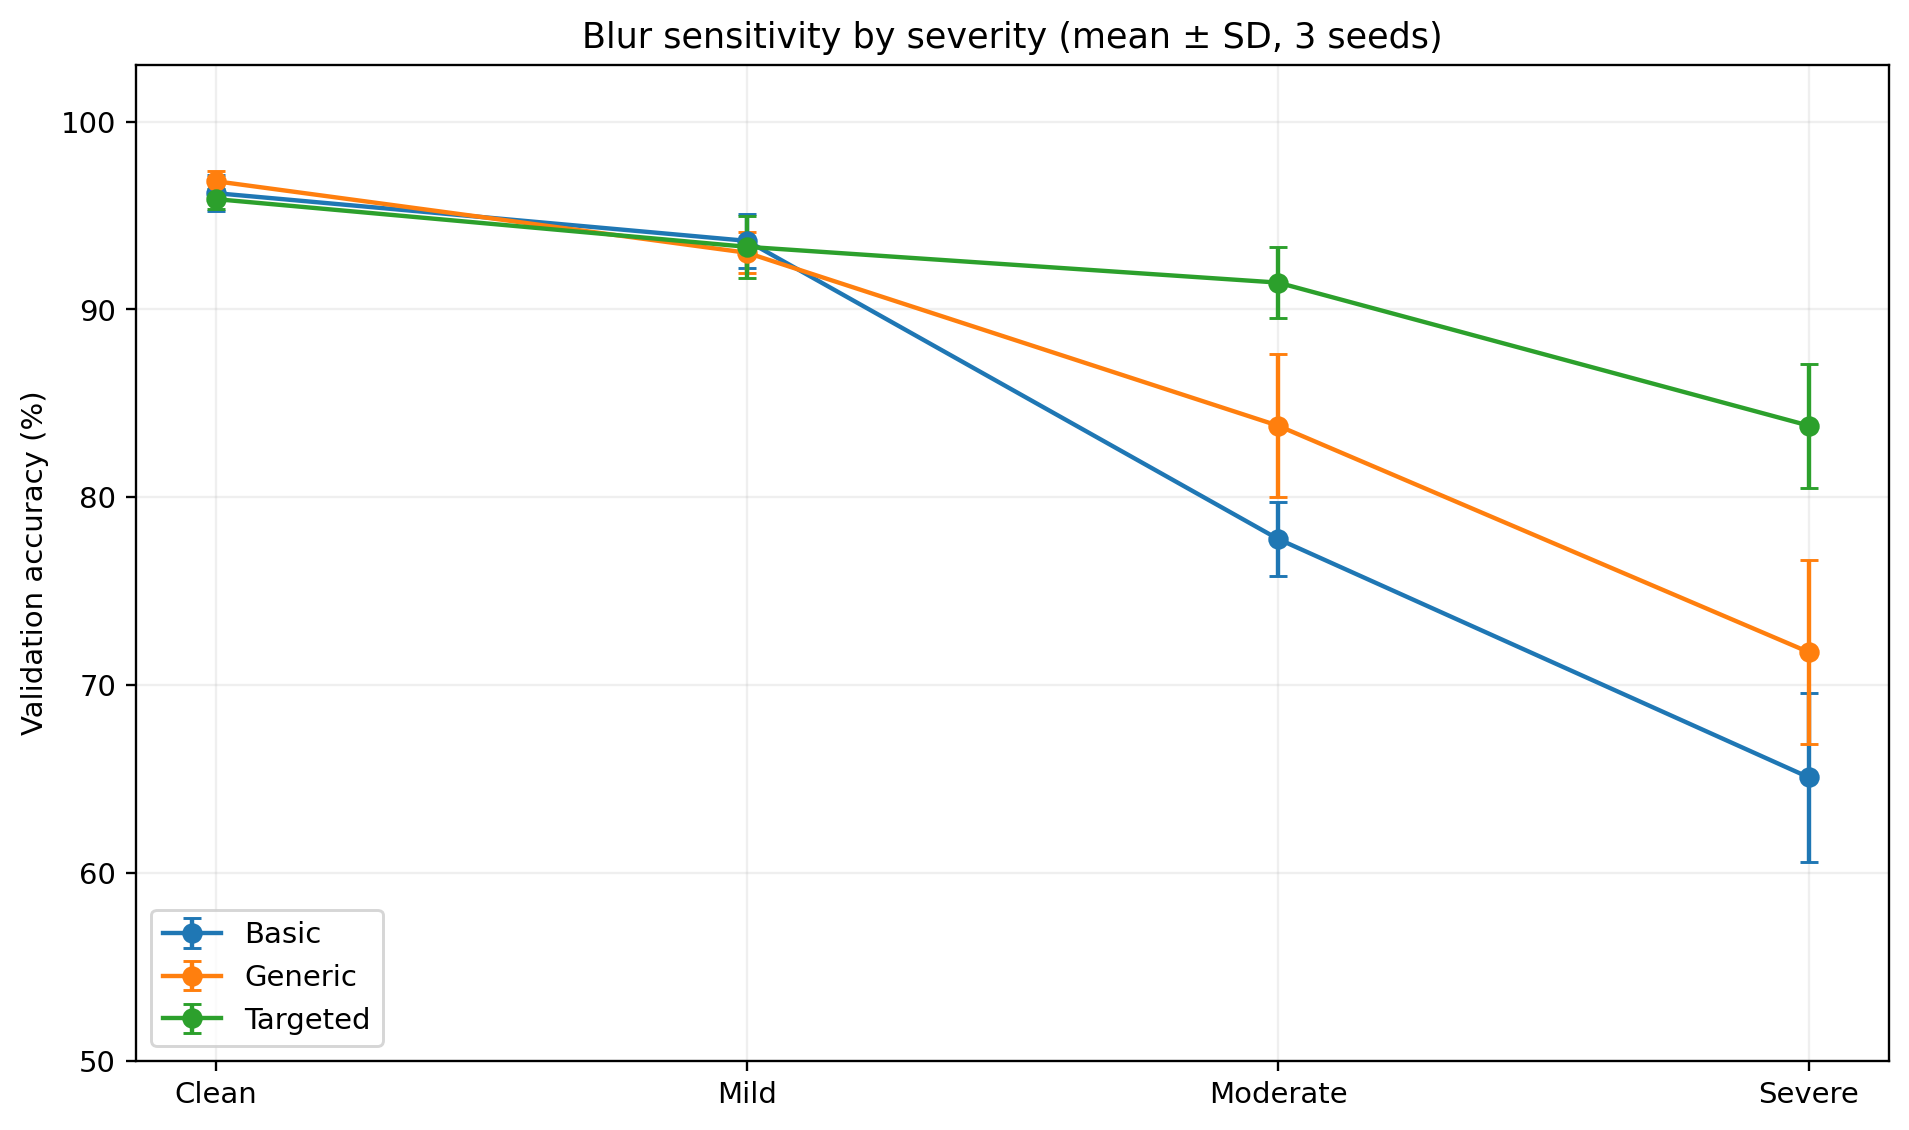
\includegraphics[width=\columnwidth]{blur_severity_curve.png}
\caption{Validation accuracy by blur severity for the three policies, averaged across the same three training seeds. Severity 0 is uncorrupted.}
\label{fig:blur}
\end{figure}

The steep blur decline shown in Fig.~\ref{fig:blur} is the strongest motivation for the final study. For RQ1 the results indicate sensitivity to corruption type and severity; for RQ2 they suggest a positive severe-blur effect but an occlusion counterexample; for RQ3 they show that a targeted robustness gain need not preserve the very highest clean accuracy. At the midterm stage these are observed \emph{validation} patterns only.


Another interpretation risk is the apparent increase in performance under mild image changes. Small positive shifts are possible because slight smoothing or brightness adjustment can interact with training preprocessing; they should not be described as proof that image corruption is beneficial in general. In the results plot, a severe-blur improvement for Targeted does not guarantee improvement for every SKU. The research plan includes class-wise confusion analysis to identify whether gains concentrate on visually simple categories, and an unseen-corruption control to reveal over-specialization to the training transform families. Those analyses are not claimed as completed midterm outcomes.

\subsection{Ethics, limitations and reproducibility}
This is a non-human-subjects secondary-image study; the images contain commercial imagery that may also include text, promotional overlays or incidental context. We document the hosted mirror, retain upstream usage restrictions, and do not redistribute raw images or pretrained model weights without checking permissions. Our public code-and-metrics repository is intended to exclude source images, image caches and personally identifying local paths. AI-assisted coding and writing are disclosed below and must be independently checked by the two authors.

The largest internal-validity threats are label ambiguity, residual near-duplicates, unobserved capture-session correlations, and comparisons of augmentation policies whose effective distortion strengths are not intrinsically matched. The current cleaned subset deliberately excludes two conflicting IDs but is not verified to be free of \emph{perceptually} identical images. The held-out validation set is used both to select checkpoints and to report performance, so these numbers can be optimistically selected. The fixed train/val division and three seeds limit independent replication; for occlusion the seed also changes the applied test mask position, which requires a fixed panel in a stronger replication. \emph{Construct validity} is limited because synthetic blur, scalar darkening and rectangular erasure are not full models of motion blur, sensor noise, low-light color cast or natural occlusion. \emph{External validity} is limited by nine mixed-product classes and only six original test images per class. This study concerns cropped-image classification and must not be generalized to detection in cluttered grocery checkout scenes.

\subsection{Feasibility, remaining timeline and author contributions}
The project has a working RTX 4090 training environment, audited image manifests, code for three augmentation policies, three-seed validation logs and plots. The remaining work is methodological quality control rather than proving the training pipeline can execute. Table~\ref{tab:plan} lists feasible next steps. Unexpected or negative outcomes will be retained; the final report will extend this midterm paper with Results, Discussion and Conclusion after the fixed official-test evaluation.

\begin{table}[t]
\caption{Outstanding activities following the November 24, 2026 pilot (proposed leads).}
\label{tab:plan}
\small
\begin{tabular}{p{0.22\columnwidth}p{0.58\columnwidth}p{0.11\columnwidth}}
\toprule
Phase & Action / evidence to deliver & Lead\\
\midrule
Nov 25 & Check ambiguous labels and near-duplicates; lock class/split version & Both\\
Nov 26 & Present pilot patterns and limitations; rehearse individual Q\&A & Both\\
Nov 27--28 & Recheck references, incorporate plots and audit log; submit ACM paper & Both\\
After midterm & Freeze corruption panels, unseen-condition check, final test once & Both\\
Final phase & Larger category-coherent subset, uncertainty and broader validity study & Both\\
\bottomrule
\end{tabular}
\end{table}

\textbf{Authors' contributions.} Abdur Rahman Ohi (22301280) and Rafi Ehtesham Mozumder (22301489) are the Group 09 authors. The specific allocation of experiments, literature verification, implementation and writing has not been independently substantiated in the provided records, so both should confirm and replace this paragraph with the actual individual contribution statement prior to submission. Both authors are responsible for checking citations, source images, measurements and scholarly claims.

\section*{Academic integrity and AI use disclosure}
OpenAI ChatGPT assisted with literature organization, experimental planning, code development/debugging, result aggregation and draft manuscript formatting. All reported measurements are taken from the group's uploaded experiment records and must be checked by the authors. AI assistance is not a substitute for reading cited sources or verifying code and data. No fabricated classifier accuracy or final-test results are reported. The authors should adjust this disclosure to match their actual coursework policy and contributions.

\bibliographystyle{ACM-Reference-Format}
\bibliography{references}
\clearpage
\appendix
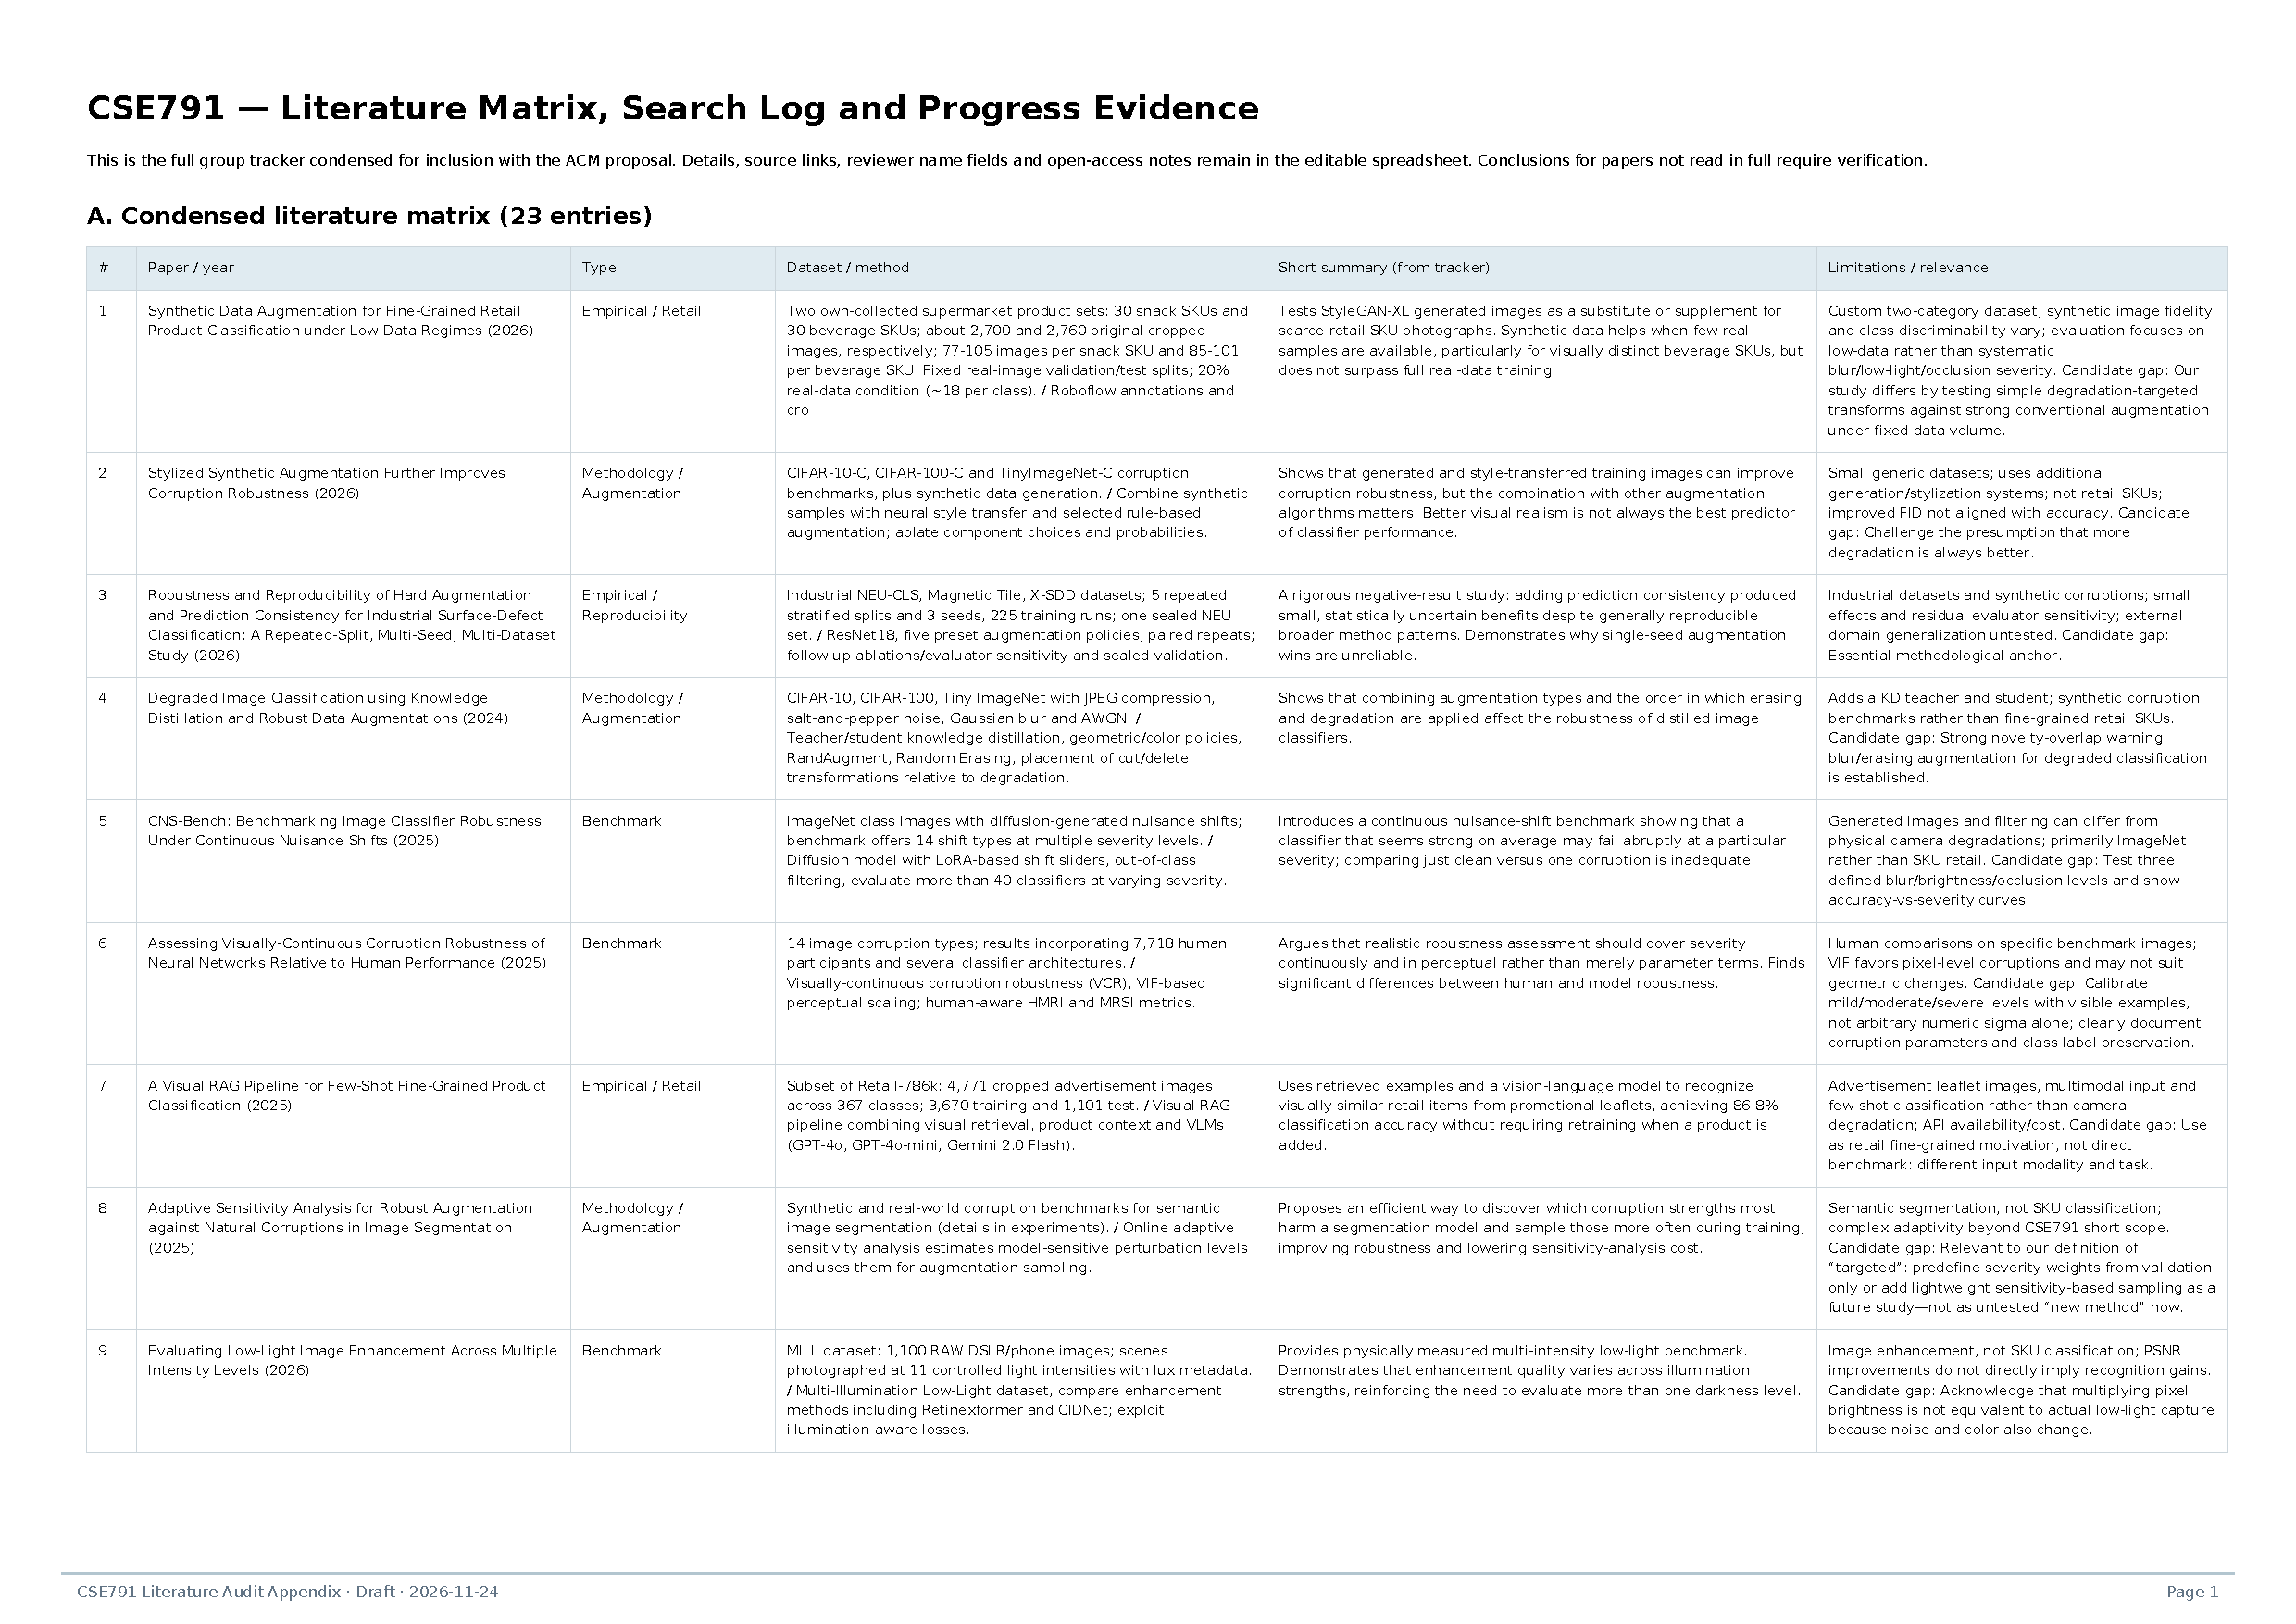
\includepdf[pages=-,fitpaper=true,pagecommand={}]{Literature_Matrix_and_Search_Log_Appendix.pdf}
\end{document}
